\section{Durchführung}
\label{sec:Durchführung}
\subsection{Aufbau und Funktionsweise des Detektors}
\label{subsec:Aufbau}
Eine schematische Skizze des verwendeten Versuchsaufbaus ist in \autoref{fig:Aufbau} zu sehen. In einem zylindrischen Gefäß befindet sich ein organisches
Szintillatormaterial. An dem linken und rechten Ende des Tanks ist jeweils ein Photomultiplier (PMT), auch Sekundärelektornenverstärker (SEV) genannt, angebracht.
Tritt ein Photon in diesen Photomultiplier ein, löst es über den äußerden Photoeffekt ein Elektron aus dem Material heraus. Dieses Elektron wird in einem elektrischen Feld 
zu einer Elektrode hin beschleunigt, wo erneut Elektronen ausgelöst werden. Dieser Prozess wiederholt sich, wobei nach jeder Beschleunigungsstufe mehr Elektronen beschleunigt werden.
Am Ende des Photomultipliers treffen die Elektronen auf eine Anode und fließen über eine Widerstand ab. Dabei ensteht ein messbarer Spannungspuls. Ein Querschnitt eines beispielhaften
Photomultipliers ist in \autoref{fig:PMT} gegeben.

Das Signal aus den beiden Photomultipliern durchläuft jeweils eine einstellbare Verzögerungsleitung und einen Diskriminator. Über die Verzögerungsleitung können eventuell unterschiedlich
schnell reagierende Photomultiplier ausgegleichen werden und über den Diskriminator wird das Signal diskretisiert und ein Rauschen wird unterdrückt. In einer Koinzidenz werden die zwei 
Signale miteindander verglichen und es wird nur ein Signal ausgegeben, wenn beide Eingangssignale zeitgleich eintreffen. Dadurch werden nur Events detektiert, die von beiden
Photomultipliern registriert werden.

Nach der Koinzidenz wird das Signal auf drei Wege aufgeteilt. Zwei Wege führen zu zwei verschiedenen AND-Gattern, ein weiterer führt durch eine $\qty{30}{\nano\second}$ Verzögerungsleitung 
zu einem Monoflop, dessen negierter Ausgang mit dem ersten AND-Gatter und der normale Ausgang mit dem zweiten AND-Gatter verbunden ist. Das Ausgangssignal des ersten AND-Gatters startet 
einen Time-Amplitude-Converter (TAC), das Signal des Zweiten stoppt diese. Mithilfe dieser Schaltung lässt sich der zeitliche Abstand zweier kurz aufeinanderfolgenden Pulse bestimmen.
Die beiden Pulse sind das Eintreten in das Szintillatormaterial und der Zerfall des Myons. Die Logik ist in \autoref{tab:Logik} tabellarisch dargestellt.

Das Signal des Time-Amplitude-Converters wird an einem Computer histogrammiert und die Daten werden zur Auswertung gespeichert.

\begin{figure}
    \centering
    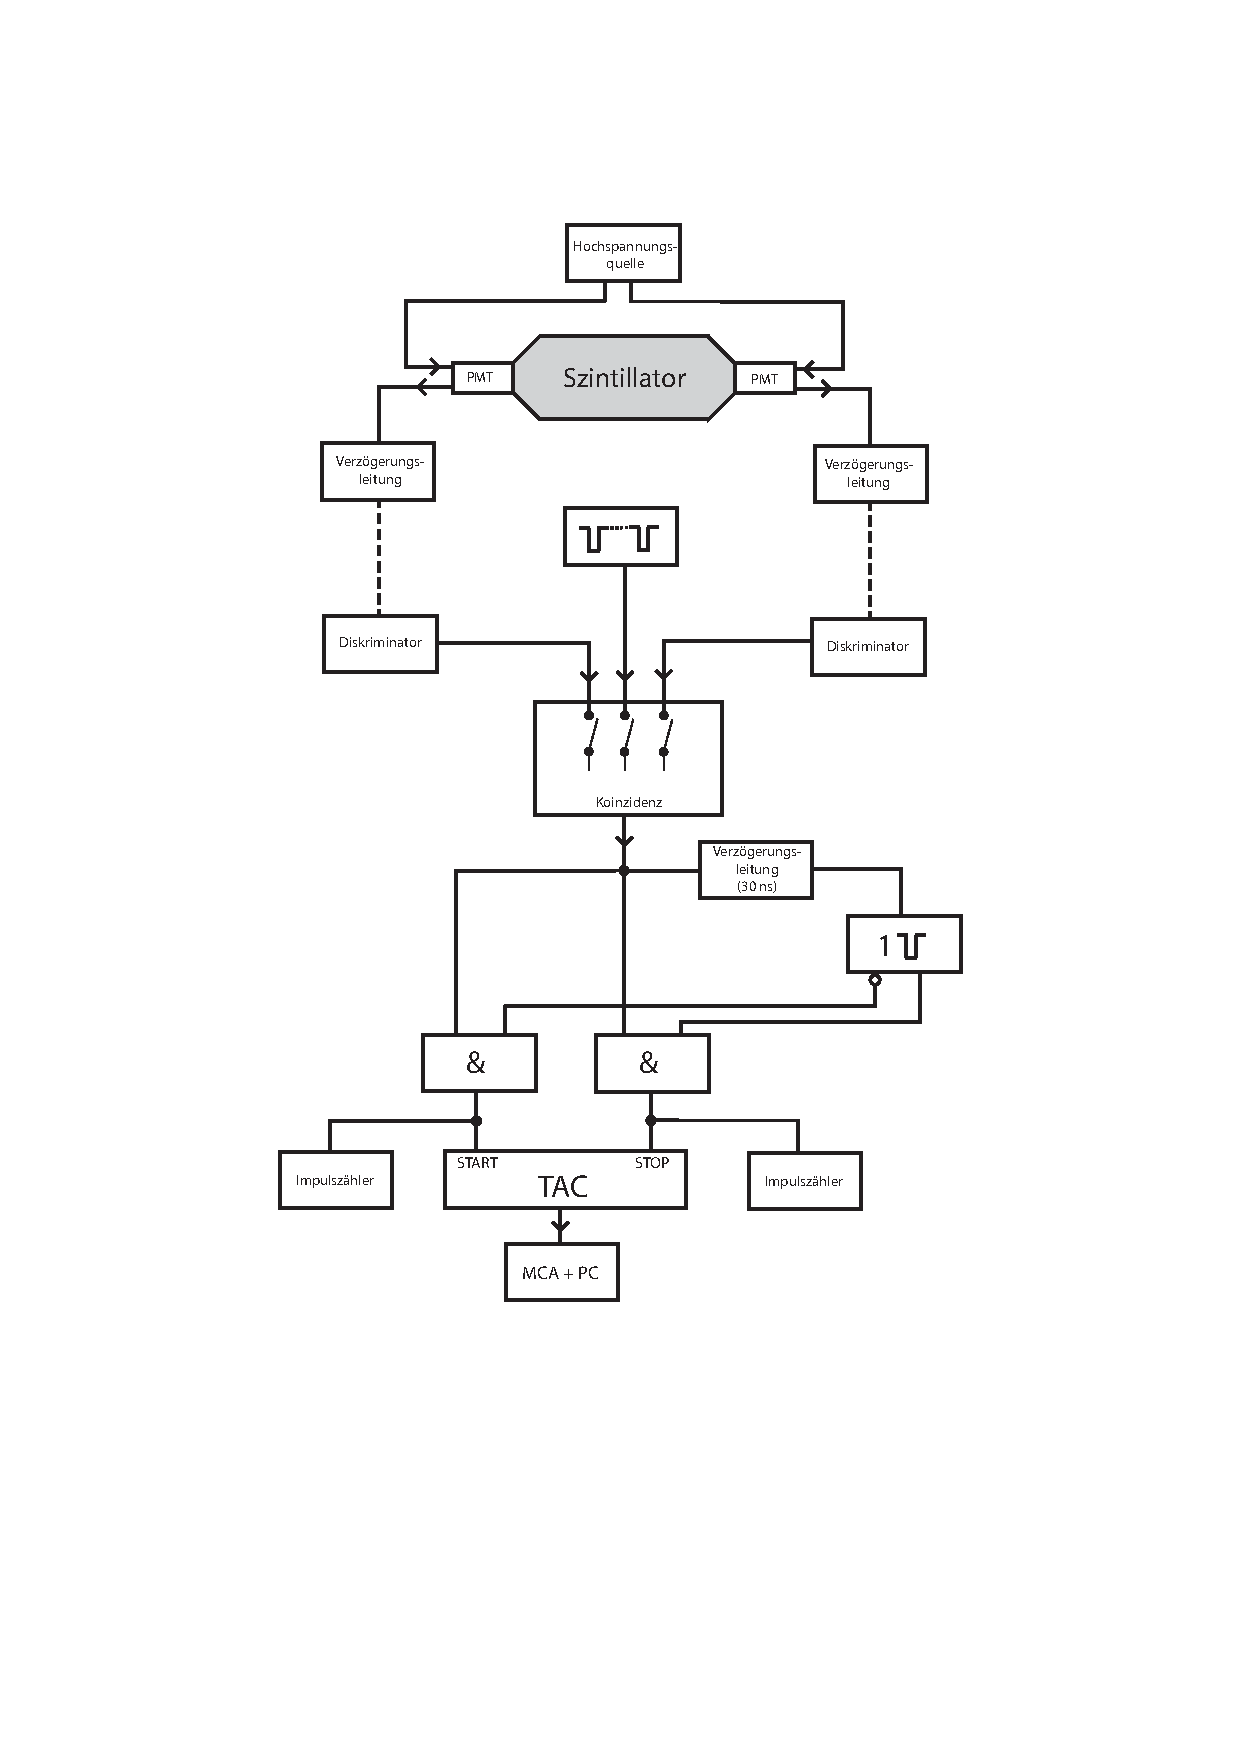
\includegraphics[width=.8\textwidth]{content/pics/Schaltbild.pdf}
    \caption{Schematische Skizze des Versuchsaufbaus. Über eine Hochspannungsquelle werden PMT betrieben, welche Photonen im Szintillatortank %
    detektieren. Das Signal durchläuft eine Verzögerungsleitung und einen Diskriminator und wird in einer Koinzidenz mit dem Signal des gegenüberliegenden PMT vergleicht. %
    Über eine analoge Logikschaltung wird ein TAC gestartet und gestoppt. Dieses Signal wird von einer Software ausgewertet \cite{V01}.}
    \label{fig:Aufbau}
  \end{figure}

\begin{figure}
    \centering
    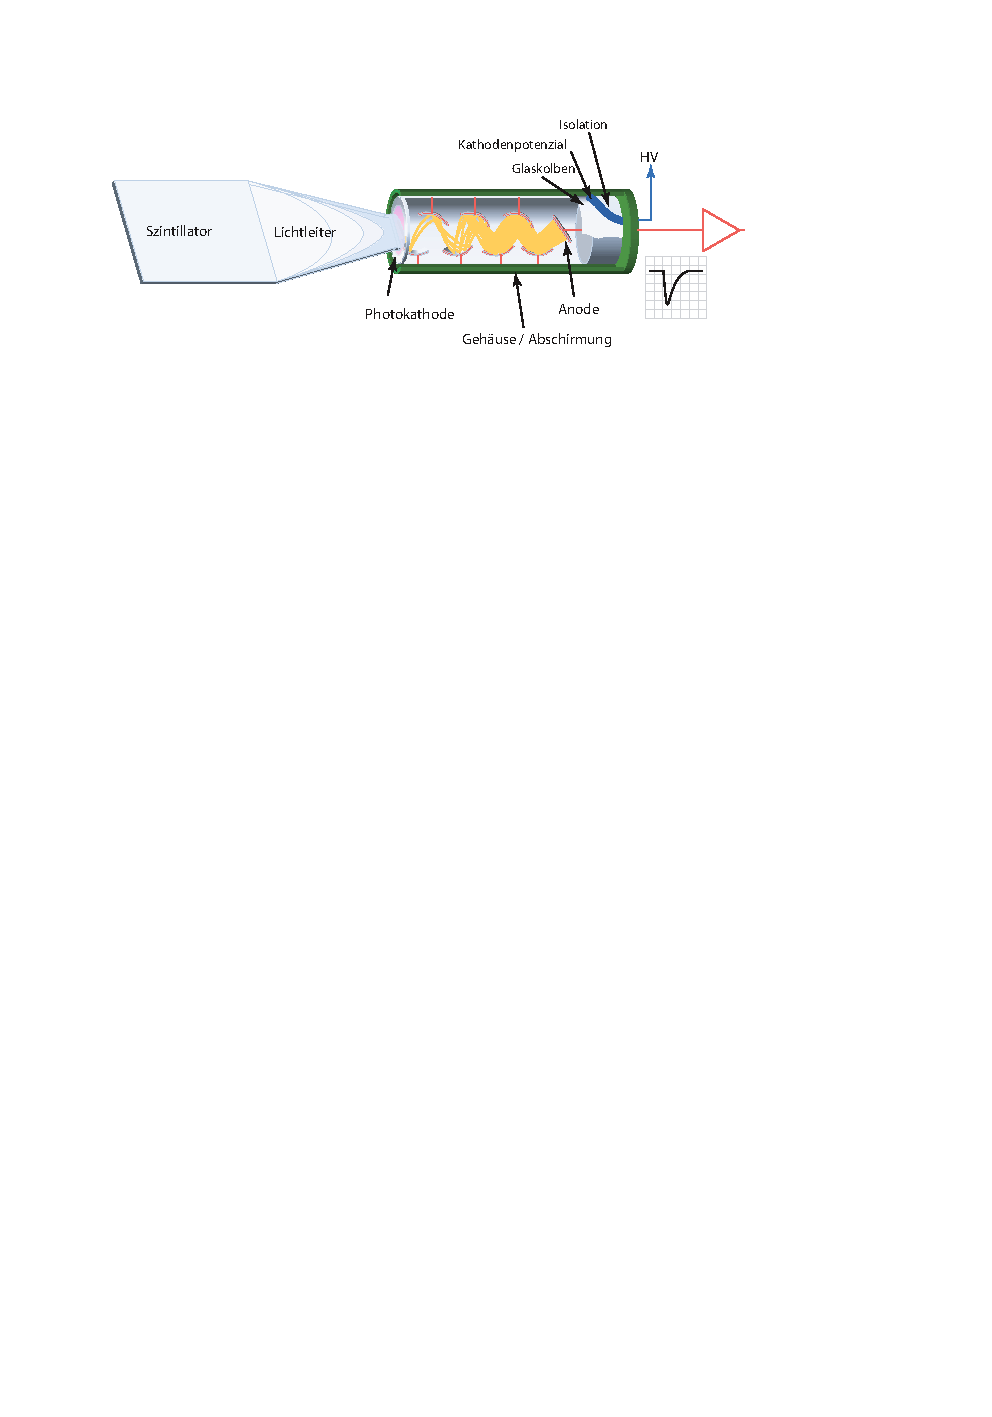
\includegraphics[width=.8\textwidth]{content/pics/PMT.pdf}
    \caption{Querschnitt eines PMT. Eintretende Photonen lösen über den äußerden Photoeffekt Elektronen aus. Die ausgelösten Elektronen werden beschleunigt und treffen erneut %
    auf ein Elektrode und lösen mehr Elektronen aus. Dies wiederholt sich, sodass am Ende des PMT ein messbarer Puls entsteht \cite{Wermes}.}
    \label{fig:PMT}
 \end{figure}


 \begin{table}
    \centering
    \caption{Logik der Schaltung des TAC. Zum Zeitpunkt $t=0$ liegt kein Signal an, bei $t=x$ und $t=x+\symup{\Delta}x$ wird gerade ein Teilchen detektiert. %
    Die Zeitdifferenz der Verzögerungsleitung beträgt $\qty{30}{\nano\second}$. In den Spalten 'Start' und 'Stopp' ist jeweils angegeben, ob die Zeitmessung %
    gestartet ist oder nicht.}
    \label{tab:Logik}
    \begin{tabular}{l | c c | c c | c c}
      \toprule
      {} & \multicolumn{2}{c|}{AND 1} & \multicolumn{2}{c|}{AND 2} & {} & {} \\
      $t$ & $1$ & $2$ & $3$ & $4$ & Start & Stopp \\
      \midrule
      $0$                                               & 0 & 1 & 0 & 0 & 0 & 1 \\
      $x$                                               & 1 & 1 & 1 & 0 & 1 & 0 \\
      {$x + \qty{30}{\nano\second}$}                    & 0 & 0 & 0 & 1 & 1 & 0 \\
      {$x + \symup{\Delta}x$}                           & 1 & 0 & 1 & 1 & 0 & 1 \\
      {$x + \symup{\Delta}x + \qty{30}{\nano\second}$}  & 0 & 1 & 0 & 0 & 0 & 1 \\      
      
      \bottomrule
    \end{tabular}
  \end{table}

  \subsection{Messung}
  \label{subsec:Messung}
  bla bla bla
